\documentclass[a4paper]{article}
\usepackage[left=3.5cm, right=3.5cm, top=2cm]{geometry}
\usepackage{tabularx} 
\renewcommand{\tabularxcolumn}[1]{m{#1}}
\usepackage{graphicx}
\graphicspath{ {./images/} }
\usepackage{multirow}
\renewcommand{\arraystretch}{1.2}
\usepackage{textcomp}

%opening
\title{\textbf{DevOps : Continuous Integration and Continuous Deployment applied} \\~\\
\large \textbf{Project Critical Review}}
\author{Hector Pascual Haba}

\begin{document}

\maketitle 

\section{General comments about the work progress}

\subsection{Incidences}

The field I am investigating and getting deeper with is a trending topic in the software area, I am not having many difficulties for finding books in which read and learn about DevOps concepts. The hard part is developing the whole application core and modules in Python, which requires time and self-learning. But due to the correct initial planning performed in which much time was spent I am now getting the results as expected, without more effort than the already planned to be dedicated.
\\~\\
I am now working as expected on subtask 2.5.2 and the previous work packages have been completed and reviewed each.
\\~\\
The only incidence that I have noticed along the development of the project is that I am dedicating less time to researching on concepts and developing the knowledge on DevOps than developing the application. But this does not alter the initial planning as there were no hours estimation performed. Moving on to the GANTT diagram, I am talking about the need of spending more time on WP 4.1 along the next weeks, so this WP's priority will upgrade.

\subsection{Clarifications regarding tasks structure}

The structure of the project tasks follows the next order :

\medskip
\textbf{Major constituent} \textrightarrow \textbf{Work Package} \textrightarrow \textbf{Sub Tasks} (if any)
\medskip\\~
Conceiving a work package as a single well-defined structure (not general or abstract as Major Constituents are) containing a notable amount of work which could include subtasks, as it is shown in the following diagram and in below tables with work packages definitions: 
\begin{center}
	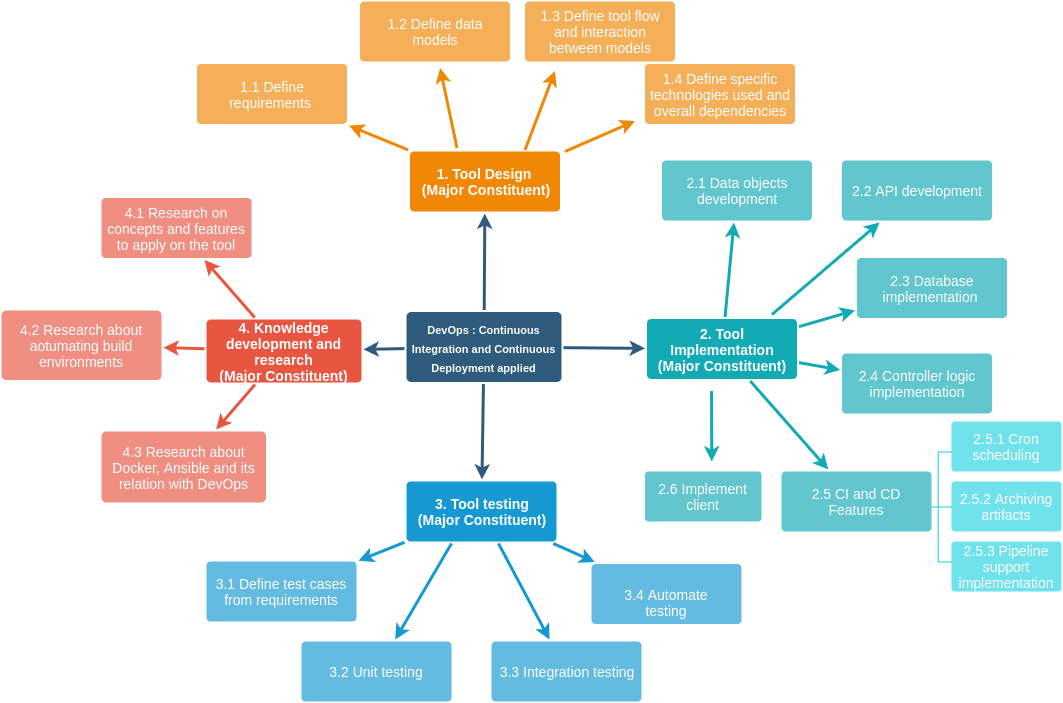
\includegraphics[scale=0.21]{wp_breakdown}
\end{center}

\newpage


\section{Updated Work Plan}

\subsection{Work Packages, Tasks and Milestones}
~\\
\begin{tabularx}{\textwidth}{|X|c|}
	\hline
	\textbf{WP Name:} Define requirements& \textbf{WP ref: 1.1} \\ \hline
	\textbf{Major constituent:} Tool Design & - \\ \hline
	\multirow{2}{*}{\begin{tabular}[c]{@{}l@{}}\textbf{Short description:} Define specific requirements\\based on DevOps real world culture and concepts \end{tabular}} &  \textbf{Planned start date:} 16/Feb/2020\\ \cline{2-2} 
	&  \textbf{Planned end date:} 19/Feb/2020\\ \hline
\end{tabularx}
\\\vspace{5px}\\
\begin{tabularx}{\textwidth}{|X|c|}
	\hline
	\textbf{WP Name:} Define data models& \textbf{WP ref: 1.2} \\ \hline
	\textbf{Major constituent:} Tool Design & - \\ \hline
	\multirow{2}{*}{\begin{tabular}[c]{@{}l@{}}\textbf{Short description:} Think about data models\\that will define the tool and its DB representation. \end{tabular}} &  \textbf{Planned start date:} 24/Feb/2020\\ \cline{2-2} 
	&  \textbf{Planned end date:} 26/Feb/2020\\ \hline
\end{tabularx}
\\\vspace{5px}\\
\begin{tabularx}{\textwidth}{|X|c|}
	\hline
	\textbf{WP Name:} Define tool flow and interaction& \textbf{WP ref: 1.3} \\ \hline
	\textbf{Major constituent:} Tool Design & - \\ \hline
	\multirow{2}{*}{\begin{tabular}[c]{@{}l@{}}\textbf{Short description:} Define the application flow\\of the application and how the models will\\interact between them.  \end{tabular}} &  \textbf{Planned start date:} 26/Feb/2020\\ \cline{2-2} 
	& \multicolumn{1}{c|}{\begin{tabular}[c]{@{}c@{}}\\\textbf{Planned end date:} 27/Feb/2020\end{tabular}}\\ & \\ \hline
\end{tabularx}
\\\vspace{5px}\\
\begin{tabularx}{\textwidth}{|X|c|}
	\hline
	\textbf{WP Name:} Define specific technologies and dependencies& \textbf{WP ref: 1.4} \\ \hline
	\textbf{Major constituent:} Tool Design & - \\ \hline
	\multirow{2}{*}{\begin{tabular}[c]{@{}l@{}}\textbf{Short description:} Define programming\\languages involved, general dependencies and\\technologies that will be used. \end{tabular}} &  \textbf{Planned start date:} 25/Feb/2020\\ \cline{2-2} 
	& \multicolumn{1}{c|}{\begin{tabular}[c]{@{}c@{}}\\\textbf{Planned end date:} 25/Feb/2020\end{tabular}} \\ 
	& \\ \hline
\end{tabularx}
\\\vspace{5px}\\
\begin{tabularx}{\textwidth}{|X|c|}
	\hline
	\textbf{WP Name:} Data objects development& \textbf{WP ref: 2.1} \\ \hline
	\textbf{Major constituent:} Tool Implementation & - \\ \hline
	\multirow{2}{*}{\begin{tabular}[c]{@{}l@{}}\textbf{Short description:} Represent the data models\\in Python class and the database models as well. \end{tabular}} &  \textbf{Planned start date:} 02/Mar/2020\\ \cline{2-2} 
	&  \textbf{Planned end date:} 05/Mar/2020\\ \hline
\end{tabularx}
\\\vspace{5px}\\
\begin{tabularx}{\textwidth}{|X|c|}
	\hline
	\textbf{WP Name:} API Developments& \textbf{WP ref: 2.2} \\ \hline
	\textbf{Major constituent:} Tool Implementation & - \\ \hline
	\multirow{2}{*}{\begin{tabular}[c]{@{}l@{}}\textbf{Short description:} Development of the API in\\order to make the models accessible from a client. \end{tabular}} &  \textbf{Planned start date:} 09/Mar/2020\\ \cline{2-2} 
	&  \textbf{Planned end date:} 24/Mar/2020\\ \hline
\end{tabularx}
\\\vspace{5px}\\
\begin{tabularx}{\textwidth}{|X|c|}
	\hline
	\textbf{WP Name:} Database Implementation& \textbf{WP ref: 2.3} \\ \hline
	\textbf{Major constituent:} Tool Implementation & - \\ \hline
	\multirow{2}{*}{\begin{tabular}[c]{@{}l@{}}\textbf{Short description:} Implement the logic for\\accessing to the SQL database using Python. \end{tabular}} &  \textbf{Planned start date:} 03/Mar/2020\\ \cline{2-2} 
	&  \textbf{Planned end date:} 10/Mar/2020\\ \hline
\end{tabularx}
\\\vspace{5px}\\
\begin{tabularx}{\textwidth}{|X|c|}
	\hline
	\textbf{WP Name:} Controller logic implementation& \textbf{WP ref: 2.4} \\ \hline
	\textbf{Major constituent:} Tool Implementation & - \\ \hline
	\multirow{3}{*}{\begin{tabular}[c]{@{}l@{}}\textbf{Short description:} Develop the logic for using\\the data models and giving capabilities for user\\interaction through the API.\end{tabular}} &  \textbf{Planned start date:} 08/Mar/2020\\ \cline{2-2} 
	& \multicolumn{1}{c|}{\begin{tabular}[c]{@{}c@{}}\\\textbf{Planned end date:} 29/Mar/2020\end{tabular}}\\ 
	&  \\ \hline
\end{tabularx}
\\\vspace{5px}\\
\begin{tabularx}{\textwidth}{|X|c|}
	\hline
	\textbf{WP Name:} CI and CD Features& \textbf{WP ref: 2.5} \\ \hline
	\textbf{Major constituent:} Tool Design & - \\ \hline
	\multirow{2}{*}{\begin{tabular}[c]{@{}l@{}}\textbf{Short description:} Basing on the research done\\in parallel in WP 4.1 implement features. \end{tabular}} &  \textbf{Planned start date:} 30/Mar/2020\\ \cline{2-2} 
	&  \textbf{Planned end date:} 22/Apr/2020\\ \hline
	\multicolumn{2}{|l|}{\begin{tabular}[c]{@{}l@{}}\textbf{2.5.1 Cron scheduling}: Implementing capability to  schedule jobs periodically with \\ cron expressions\end{tabular}} \\ \hline
	\multicolumn{2}{|l|}{\begin{tabular}[c]{@{}l@{}}\textbf{2.5.2 Archiving artifacts}: Implementing capability to store binaries and outputs\\from build executions\end{tabular}} \\ \hline
	\multicolumn{2}{|l|}{\begin{tabular}[c]{@{}l@{}}\textbf{2.5.3 Pipeline support}: Implementing capability to define builds through YAML \\pipelines.\end{tabular}} \\ \hline
\end{tabularx}
\\\vspace{5px}\\
\begin{tabularx}{\textwidth}{|X|c|}
	\hline
	\textbf{WP Name:} Implement Client& \textbf{WP ref: 2.6} \\ \hline
	\textbf{Major constituent:} Tool Implementation & - \\ \hline
	\multirow{2}{*}{\begin{tabular}[c]{@{}l@{}}\textbf{Short description:} Implement a client with GUI\\in order to interact with the API.\end{tabular}} &  \textbf{Planned start date:}24/Apr/2020\\ \cline{2-2} 
	&  \textbf{Planned end date:} 20/May/2020\\ \hline
\end{tabularx}
\\\vspace{5px}\\
\begin{tabularx}{\textwidth}{|X|c|}
	\hline
	\textbf{WP Name:} Define test cases from requirements& \textbf{WP ref: 3.1} \\ \hline
	\textbf{Major constituent:} Tool Testing & - \\ \hline
	\multirow{2}{*}{\begin{tabular}[c]{@{}l@{}}\textbf{Short description:} Define test cases based on\\the requirements defined on WP 1.1 \end{tabular}} &  \textbf{Planned start date:} 21/May/2020\\ \cline{2-2} 
	&  \textbf{Planned end date:} 25/May/2020\\ \hline
\end{tabularx}
\\\vspace{5px}\\
\begin{tabularx}{\textwidth}{|X|c|}
	\hline
	\textbf{WP Name:} Unit tests& \textbf{WP ref: 3.2} \\ \hline
	\textbf{Major constituent:} Tool Testing & - \\ \hline
	\multirow{2}{*}{\begin{tabular}[c]{@{}l@{}}\textbf{Short description:} Write unit tests for each\\module and function that is critical. \end{tabular}} &  \textbf{Planned start date:} 25/May/2020\\ \cline{2-2} 
	&  \textbf{Planned end date:} 27/May/2020\\ \hline
\end{tabularx}
\\\vspace{5px}\\
\begin{tabularx}{\textwidth}{|X|c|}
	\hline
	\textbf{WP Name:} Integration Testing& \textbf{WP ref: 3.3} \\ \hline
	\textbf{Major constituent:} Tool Testing & - \\ \hline
	\multirow{2}{*}{\begin{tabular}[c]{@{}l@{}}\textbf{Short description:} Write integration tests\\checking overall tool functionality. \end{tabular}} &  \textbf{Planned start date:} 27/May/2020\\ \cline{2-2} 
	&  \textbf{Planned end date:} 29/May/2020\\ \hline
\end{tabularx}
\\\vspace{5px}\\
\begin{tabularx}{\textwidth}{|X|c|}
	\hline
	\textbf{WP Name:} Automate testing& \textbf{WP ref: 3.4} \\ \hline
	\textbf{Major constituent:} Tool Testing & - \\ \hline
	\multirow{2}{*}{\begin{tabular}[c]{@{}l@{}}\textbf{Short description:} Automate testing to be\\executed when merges to master are done. \end{tabular}} &  \textbf{Planned start date:} 01/Jun/2020\\ \cline{2-2} 
	&  \textbf{Planned end date:} 04/Jun/2020\\ \hline
\end{tabularx}
\\\vspace{5px}\\
\begin{tabularx}{\textwidth}{|X|c|}
	\hline
	\textbf{WP Name:} Research on concepts and features to apply on the tool& \textbf{WP ref: 4.1} \\ \hline
	\textbf{Major constituent:} Knowledge development and research & - \\ \hline
	\multirow{2}{*}{\begin{tabular}[c]{@{}l@{}}\textbf{Short description:} Read books and articles\\trending on the topic to conclude features that \\ might fit on the tool. \end{tabular}} &  \textbf{Planned start date:} 10/Mar/2020\\ \cline{2-2} 
	&  \multicolumn{1}{c|}{\begin{tabular}[c]{@{}c@{}}\\\textbf{Planned end date:} 04/Jun/2020\end{tabular}} \\
	& \\ \hline
\end{tabularx}
\\\vspace{5px}\\
\begin{tabularx}{\textwidth}{|X|c|}
	\hline
	\textbf{WP Name:} Research about automating build environments & \textbf{WP ref: 4.2} \\ \hline
	\textbf{Major constituent:} Knowledge development and research & - \\ \hline
	\multirow{2}{*}{\begin{tabular}[c]{@{}l@{}}\textbf{Short description:} Strictly related to 4.3, get\\conclusions on this topic and write thoughts. \end{tabular}} &  \textbf{Planned start date:} 11/May/2020\\ \cline{2-2} 
	&  \multicolumn{1}{c|}{\begin{tabular}[c]{@{}c@{}}\\\textbf{Planned end date:}
			01/Jun/2020\end{tabular}}\\ 
	& \\\hline
\end{tabularx}
\\\vspace{5px}\\
\begin{tabularx}{\textwidth}{|X|c|}
	\hline
	\textbf{WP Name:} Research about Docker, Ansible and its relation with DevOps& \textbf{WP ref: 4.3} \\ \hline
	\textbf{Major constituent:} Knowledge development and research & - \\ \hline
	\multirow{2}{*}{\begin{tabular}[c]{@{}l@{}}\textbf{Short description:} Research and write ways in\\which these technologies can be used and applied. \end{tabular}} & \textbf{Planned start date:} 14/May/2020\\ \cline{2-2} 
	&  \textbf{Planned end date:} 02/Jun/2020\\ \hline
\end{tabularx}
\subsection{Time Plan (Gantt diagram)}

\begin{figure}[h]
	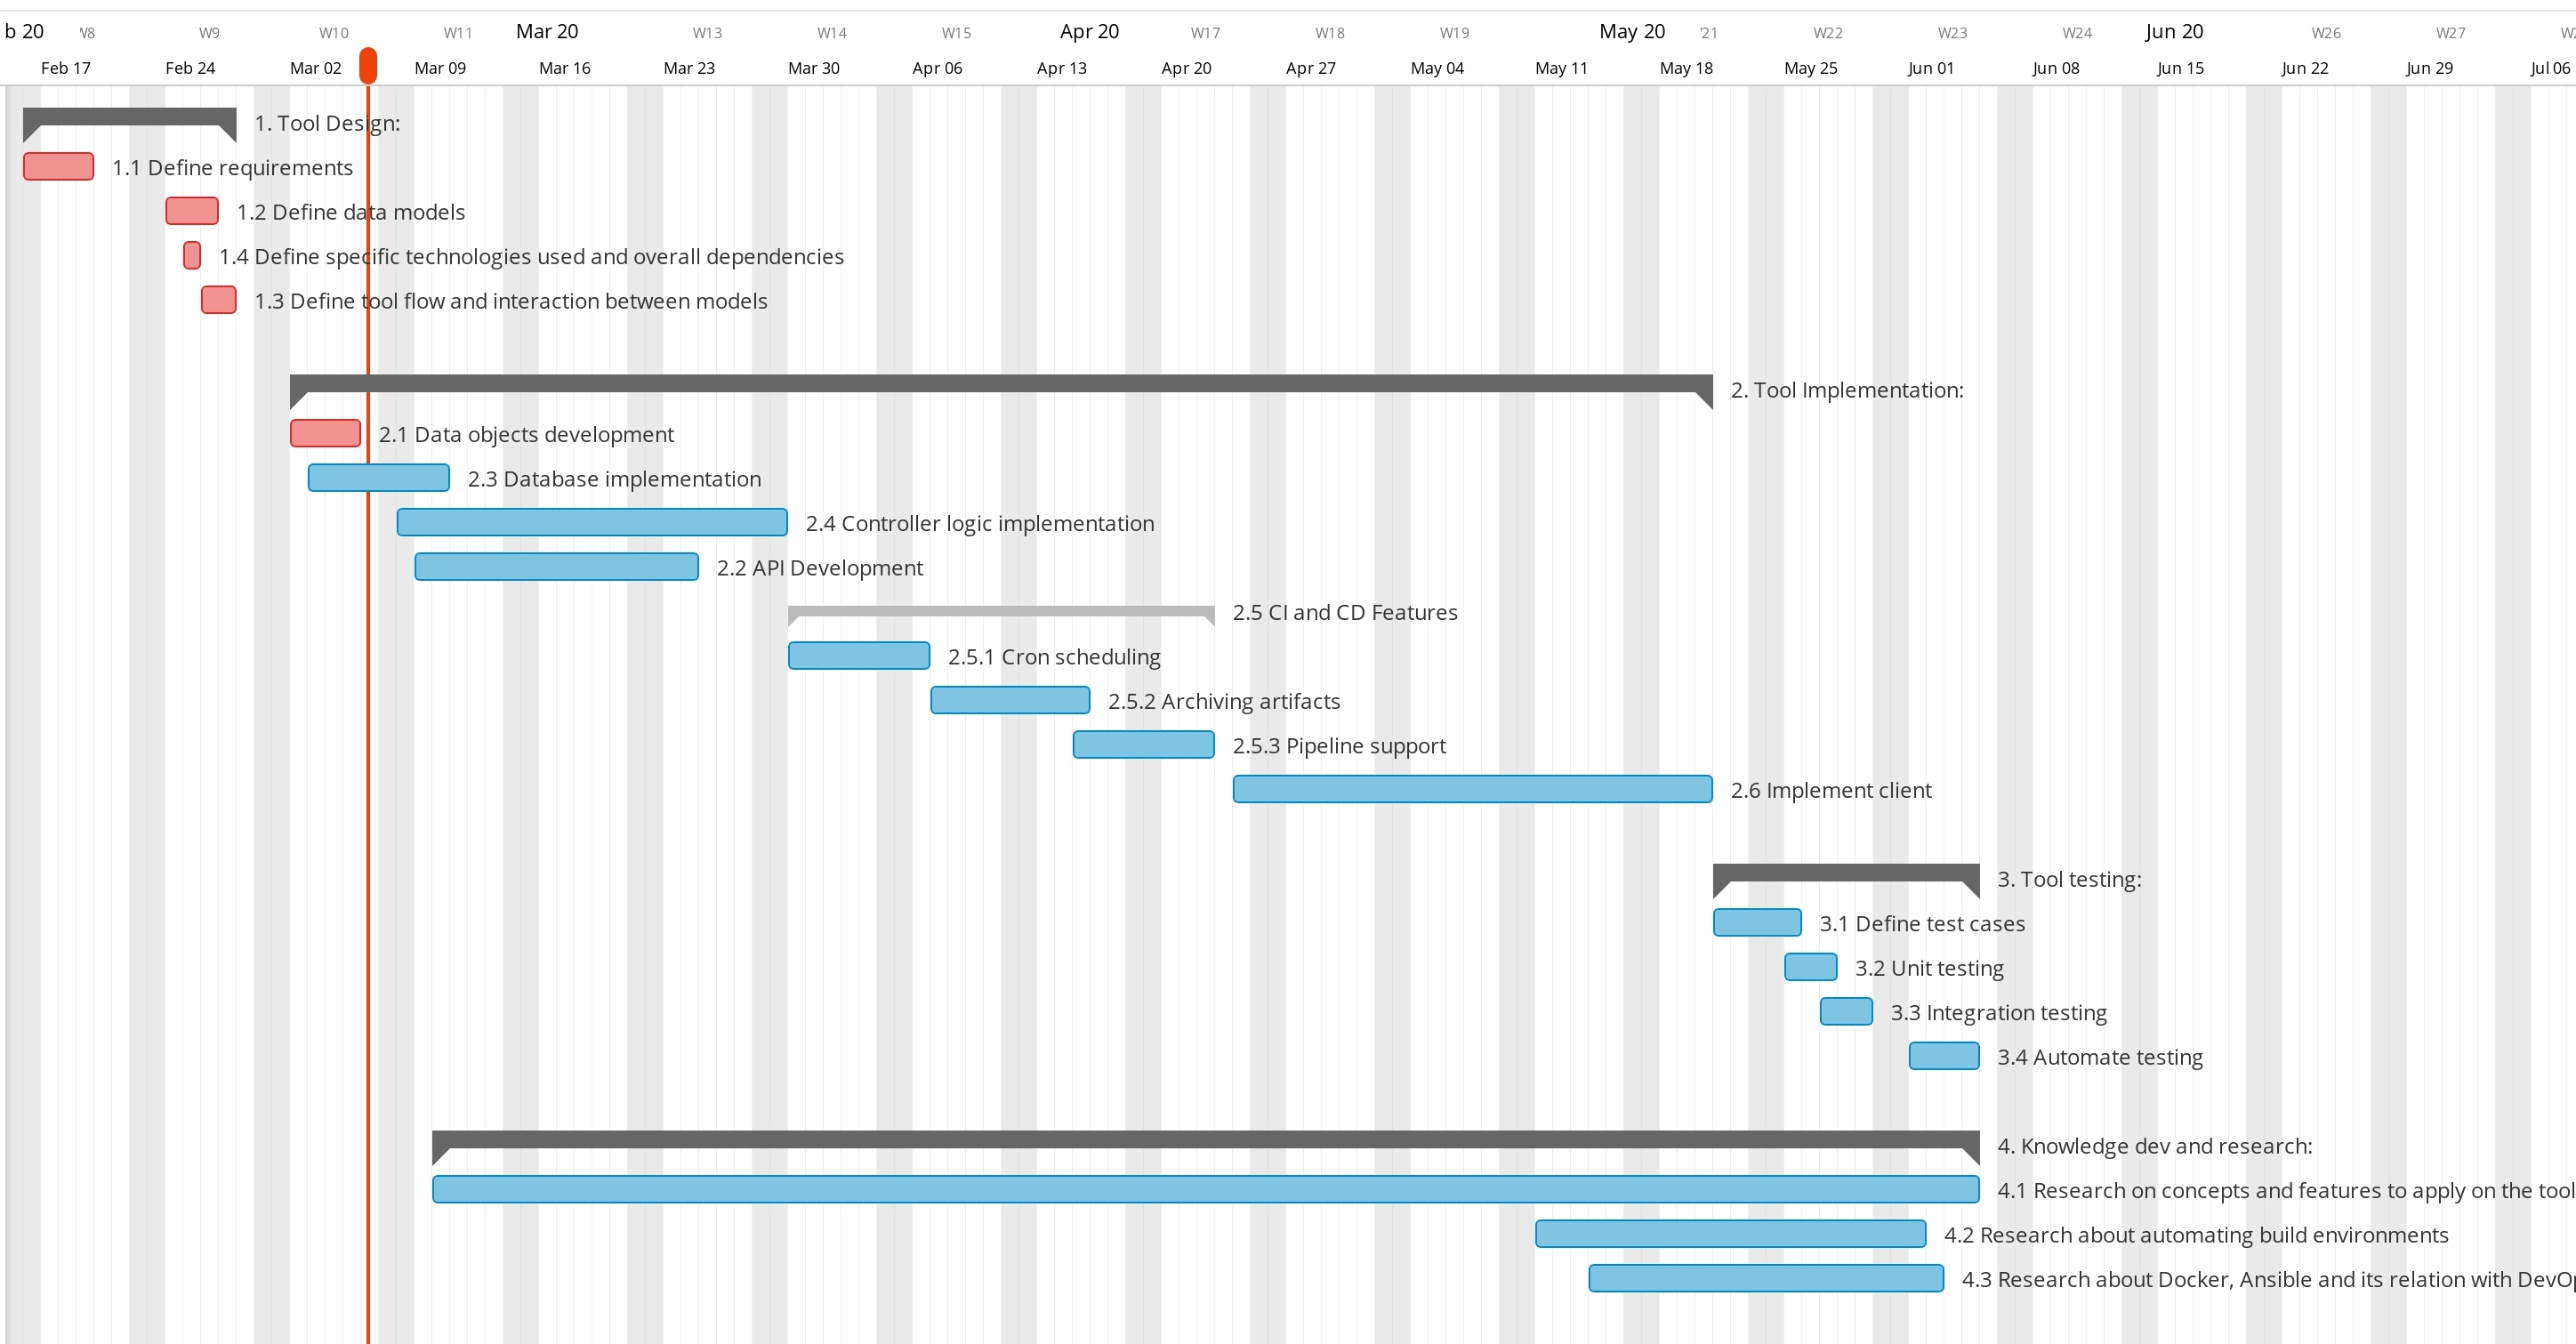
\includegraphics[scale=0.15]{gantt}
\end{figure}
\newpage

\end{document}
